\documentclass[a4paper]{article}

%%%%%%%% CREATE DOCUMENT STRUCTURE %%%%%%%%
%% Language and font encodings
\usepackage[english]{babel}
\usepackage[utf8x]{inputenc}
\usepackage[T1]{fontenc}
%\usepackage{subfig}

%% Sets page size and margins
\usepackage[a4paper,top=3cm,bottom=2cm,left=2cm,right=2cm,marginparwidth=1.75cm]{geometry}

%% Useful packages
\usepackage{amsmath}
\usepackage{graphicx}
\usepackage[colorinlistoftodos]{todonotes}
\usepackage[colorlinks=true, allcolors=blue]{hyperref}
%\usepackage{caption}
\usepackage[justification=centering]{caption}
\usepackage{subcaption}
\usepackage{sectsty}
\usepackage{float}
\usepackage{titling} 
\usepackage{blindtext}
\usepackage[square,sort,comma,numbers]{natbib}
\usepackage[colorinlistoftodos]{todonotes}
\usepackage{xcolor}
\usepackage{fancyhdr}
\usepackage{lipsum}

%% definitions 
\definecolor{darkgreen}{rgb}{0.0, 0.4, 0.0}

%% Define your personal info here %%%%%%%%%%%%%%%%%%%%%%%
\newcommand\TPid{0}
\newcommand\TPname{Stohastic processes}
\newcommand\Firstname{Joao Filipe}
\newcommand\Familyname{Costa da Quinta}
\newcommand\Email{Joao.Costa@etu.unige.ch}

%%%%%%%%%%%%%%%%%%%%%%%%%%%%%%%%%%%%%%%%%%%%%%%%%%%%%%%

%%%%%%% Page header %%%%%%
\pagestyle{fancy}
\fancyhf{}
\rhead{TP \TPid: \TPname}
\lhead{\Firstname \Familyname}
\rfoot{Page \thepage}


%%%%%%%% DOCUMENT %%%%%%%%
\begin{document}

%%%% Title Page
\begin{titlepage}

\newcommand{\HRule}{\rule{\linewidth}{0.5mm}} 							% horizontal line and its thickness

\center 
 
% University
\textsc{\LARGE Université de Genève}\\[1cm]

% Document info
\textsc{\Large Metaheuristics for optimization}\\[0.2cm]									% Course Code
\HRule \\[0.8cm]
{ \huge \bfseries TP \TPid : \TPname}\\[0.7cm]								% Assignment
\HRule \\[2cm]
\large
\emph{Author:} \Firstname \; \Familyname\\[0.5cm]		
\emph{E-mail:} {\color{blue}\Email}\\[7cm]		
% Author info
% Author info
{\large \today}\\[2cm]

\includegraphics[width=0.4\textwidth]{images/unige_csd.png}\\[1cm] 	% University logo
\vfill 
\end{titlepage}


% ============================================
% ----------------------------------
\section*{Simulation of a balanced dice}
\subsection*{Intro}
During this exercise we will be simulating rolls of a N-face balanced dice. This means that the dice has N possible outcomes at each throw, all faces are equally likely with a probability of 1/N.\\
For each roll we need to do the following three tasks:
\begin{itemize}
\item [(1)] compute a new random value $r \in [0,1)$, done with random() function from random package
\item [(2)] compute $i = N * r$
\item [(3)] compute $\lfloor i \rfloor$, done with floor() function from math package
\end{itemize}
After doing the three tasks, we get a value, that is the simulated roll.\\
The following graphic represents this phenomenon for N = {6, 15}\\
\begin{figure}[H]
\center
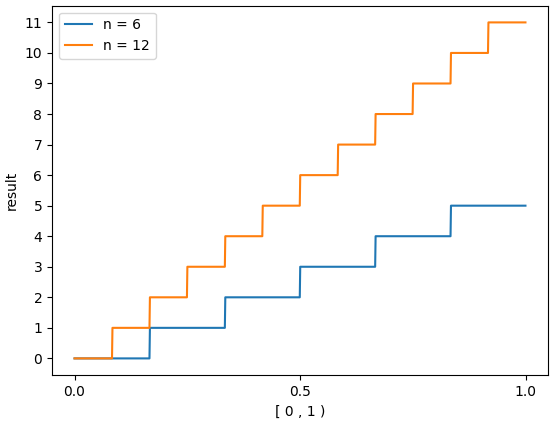
\includegraphics[width=0.5\textwidth]{images/balanced_dice.PNG}
\caption{Values for N = $\{6, 12\}$}
\end{figure}
In the image above we see this kind of step function, this is due to the fact that we use the function .floor().\\
The function that does this computation can be found in the functions.py file, and its signature is the following:
\begin{center}
balancedDice(N), where N corresponds to the number of faces in the balanced dice.
\end{center}
To check if the function works well we simply use it a large amount of times, or n times, if all faces are represented the same amount of times we know it is a good simulation. Obviously we need n to be large enough.
\subsection*{Results}
For our results we will run the script with N = 6, and n = $\{ 100, 1000, 10000\}$.\\
To 'read' the results, we will be computing the frequency of each face. Let's say the face represented by the value 1 was seen 20 times out of 100 rolls, then its frequency is 20/100 = 0.2.
\begin{center}


\begin{table}[H]
\begin{tabular}{|c|c|c|c|c|c|c|}
\hline
Face                   & 1      & 2     & 3      & 4      & 5      & 6      \\ \hline
Frequency: 100 rolls   & 0.18   & 0.21  & 0.15   & 0.18   & 0.15   & 0.13   \\ \hline
Frequency: 1000 rolls  & 0.184  & 0.17  & 0.148  & 0.165  & 0.167  & 0.166  \\ \hline
Frequency: 10000 rolls & 0.1742 & 0.167 & 0.1671 & 0.1663 & 0.1641 & 0.1613 \\ \hline
\end{tabular}
\end{table}
\end{center}






% ----------------------------------
\section*{Discrete Case}

\end{document}
